% Chaper background Continued .. 
\section{Recommender System}
Recommender systems are information filtering systems that provide a solution for the problem of information overload \cite{45}. The process involves filtering important information out of a large amount of data according to the user's preferences and interests. The recommender systems can predict item or product relevancy to the user based on the user's profile and preferences. The basic idea of the general recommender model is given in \autoref{fig:recommender_model} \\ which explains the interaction of users and items with the system. Dataset of items represents the description of items for instance recipes. Description of a recipe may contain information about different factors of recipes such as ingredients used in the recipe, cooking type, calories, cuisine type. Consider a user who likes Mexican recipes with low calories. The profile exploitation step matches the user's profile information with all recipes present in the data set. At this point, the recommendation algorithm gets applied to match the user profile and recipe profile. All Mexican dishes with low calories will get filtered out from the data set for our user. All filtered recipes hold some ranking based on the recommendation algorithm. Top- N recipes will get recommended to our user based on the ranking predicted by the recommendation algorithm. The user adopts those recommendations and responds to the results generated by the recommendation system by providing feedback. The system updates the user profile based on the feedback received by the system from a user. Recommendation systems correlate one user with a group of other users to find similar users. In this case, the system will match a user's profile with all other users who prefer Mexican low-calorie food. 

\begin{figure}[H]
	\centering
	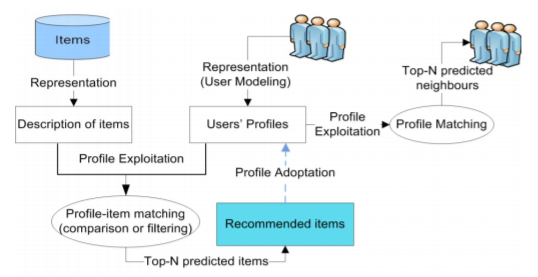
\includegraphics[width=0.7\linewidth]{recommender_model}
	\caption{General Recommender Model \cite{3}}
	\label{fig:recommender_model}
\end{figure}

\noindent Based on recommendations generated by the system, interaction between users and items may vary. For that reason, we need to understand the features of different recommendation techniques. \autoref{fig:recommender_techniques} shows broadly categorized recommendation techniques.

\begin{figure}[H]
	\centering
	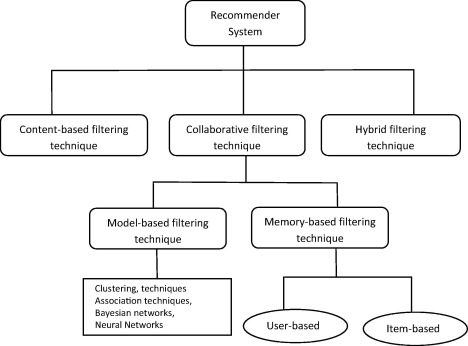
\includegraphics[width=0.7\linewidth]{recommender_techniques}
	\caption{Recommendation Techniques \cite{33}}
	\label{fig:recommender_techniques}
\end{figure}


\noindent As shown in \autoref{fig:recommender_techniques}, traditionally there are two basic models of recommender systems. \begin{itemize} \item Content Based Filtering \item Collaborative Filtering \end{itemize}
These commonly used filtering approaches are discussed in the next section.
\pagebreak

\subsection{Content Based Filtering}
In the Content-based method algorithm, user preference is considered based on the item description. The rating and buying behavior of users are combined with content information available in the items. The main aim of content-based filtering is to create a profile for each item as well as each user in order to find similar items that reflect a user's taste \cite{6}.
\\

\begin{figure}[H]
	\centering
	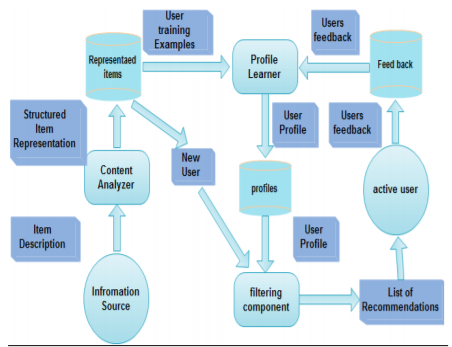
\includegraphics[width=0.7\linewidth]{contentbased_architecture}
	\caption{Content Based filtering Architecture \cite{5}}
	\label{fig:contentbased_architecture}
\end{figure}

\noindent 
The architecture of content based model highlights the process in \autoref{fig:contentbased_architecture}. 


\begin{itemize}
\item \textbf{Content Analyzer} 
\\
When information has no exact structure, the pre-processing step is necessary to extract relevant features from that document. Content analyzer analyzes items such as recipes, documents, books, product descriptions to extract and present the content of items. Information source contains data in the raw format. Each data item coming from an information source is pre-processed and analyzed by feature extraction techniques to transform original information into a more structured format. The output of the content analyzer is the input for the profile learner and filtering component.

\item \textbf{Profile Learner} 
\\
Profile learner constructs a user profile by collecting user preference data. The generalization strategy is applied to the collected data using machine learning techniques. For example, the profile learner of a movie recommender can implement a relevance feedback method in which rating on a scale of 0 to 5 is considered. Rating value above 3 is considered as a positive rating implies likes for the movie and rating value below 3 considered as negative rating implies dislike for a movie. The learning technique combines liked and disliked movies by the user and the vector of positive and negative examples into a vector that represents user profile. 

\item \textbf{Filtering Component}
\\
The filtering component uses the user's profile to find matching items from the items' data set. The items are matching with a user's data profile are decided by calculating the similarity between a user's data profile and item vectors. A list of potentially interesting items is recommended by the filtering component. 
\end{itemize}
\noindent
In a content-based algorithm, each user's information can be stored in vector form which contains past behavior of the user. This vector is known as user vector or user profile. All the information about an item is stored in an item vector or item profile which contains all the details about item-specific attributes. Based on the similarity score between the user profile and item profile most relevant items are recommended to the user. The calculation of user or item vector is discussed in section \nameref{vector_space_model}.

\subsubsection{Vector Space Model}
\label{vector_space_model}
Vector Space Model (VSM) for information retrieval represents documents as queries as vectors of weight \cite{46}. It is also known as the term vector model as it uses term occurrences as a vector identifier. 
\\
Each item profile and user profile can be represented in the form of vectors. For instance, consider an example of users and books rating relationships based on ratings given by users to books based on the book's genre. The \autoref{book_genre} represents the book and its genre relationship in binary form. Here, 1 is considered as book shares that genre and 0 represent that book does not share the genre. Book1 is solely based on Machine Learning while book3 talks about Security and Databases. Here, the genre of book is an attribute or feature that is considered to represent a book in vector form. Rows in \autoref{book_genre} represents item vector for book1, book2 and book3 respectively.   

\begin{table}[]
\centering

\begin{tabular}{|l|l|l|l|}
\hline
      & Machine Learning & Databases & Cyber Security \\ \hline
book1 & 1                & 0         & 0              \\ \hline
book2 & 1                & 0         & 1              \\ \hline
book3 & 0                & 1         & 1              \\ \hline
\end{tabular}
\caption{Books in Vector Form}

\label{book_genre}
\end{table} 

\noindent
Similarly, a user profile can be represented in a vector form. Consider a user liked book1 and book3 where 1 represents like and 0 represents dislike as shown in \autoref{user_ratings_for_books}. 

\begin{table}[]
\centering
\begin{tabular}{|l|l|}
\hline
      & user ratings \\ \hline
book1 & 1            \\ \hline
book2 & 0            \\ \hline
book3 & 1            \\ \hline
\end{tabular}
\caption{User Rating for Books}
\label{user_ratings_for_books}
\end{table}

\noindent The simplest way to form a user vector is to take a sum of dot product of matrices as resulted in \autoref{book_user_vector}.  
\begin{table}[]
\centering
\begin{tabular}{|l|l|l|}
\hline
Machine Learning & Databases & Cyber Security \\ \hline
1                & 1         & 1              \\ \hline
\end{tabular}
\caption{User Vector for Book's Genres}
\label{book_user_vector}
\end{table}

\noindent The content of an item can be complex such as text containing many words with high frequency. In such cases, a binary representation of rating considers all terms with the same weight. To consider only important terms, various components are combined to calculate the weight of the term. One way to calculate the weight of a term is to use term frequencies and inverse document frequencies (TF-IDF).


\subsubsection{Term Frequency - Inverse Document Frequency (TF-IDF)}
\label{sec:tf-idf}
TF-IDF is the most common computation used in text analysis and information retrieval process. It is used to measure the importance of a term with respect to document corpus. TF-IDF weighting negates the effect of high-frequency words in order to understand the importance of the term \cite{47}. It consists of two parts, the first is `term frequency' and the second is `inverse document frequency'. The term frequency of term $i$ in a document $j$ is given in \autoref{eq:tf}
\begin{equation}
TF_{ij} = \frac{N_{i,j}}{\sum_{k} N_{kj}} = \frac{\textrm{Number of appearances of a term in a document}}{\textrm{Total number of terms in a document}}
\label{eq:tf}
\end{equation}
\noindent Where $N_{i,j}$ is a number of occurrences of term $T_{i}$ in the document $d_j$. The summation in the denominator provides the number of occurrences of all terms in the document $d_j$.
\\
\noindent Inverse document frequency computes the importance of a word by comparing its occurrence in other documents. Inverse document frequency is given in \autoref{eq:idf}
\begin{equation}
IDF_{ij} =\log \frac{\vert D \vert}{\vert\{j:T_i \in d_j \} \vert} = \frac{\textrm{Total number of documents in the corpus}}{\textrm{Number of documents appear with a term}}
\label{eq:idf}
\end{equation}
\noindent Where, $\vert D \vert$ represents the corpus of documents. Denominator gives number of documents containing the term $T_i$.
\\
\mathchardef\mhyphen="2D
\begin{equation}
TF\mhyphen IDF = TF * IDF
\label{eq:tfidf}
\end{equation}
\noindent The value of TF-IDF is calculated by multiplying value of term frequency and value of inverse document frequency. Consider an example of 100 documents corpus and a document $X$ contains 100 terms in it. The term `excellent' appears in a document $X$ 10 times. then term frequency of $X = \frac{10}{100} = 0.1$. If the term `excellent' appears in 20 different documents then $IDF = log\frac{100}{20} = 1.60. $ TF-IDF of the term `excellent' = $0.1 * 1.60 = 0.160 $


\subsubsection{Advantages of content-based filtering}

Content-based recommender systems are heavily reliant on the contents of the items that have been rated by the user. So, while making recommendations, this approach considers a user's taste and accordingly recommends an item that matches the user's preferences. Generally, the most popular items dominate less popular items. But this approach will not miss less popular items if it matches the user's unique taste \cite{6}. \\
Consider pepperoni pizza is the most popular dish and veggie pizza is a less popular dish in a restaurant. The restaurant will always recommend pepperoni pizza to every person because the dish is popular with no understanding if a customer is vegetarian or not. The content-based system analyzes that only veg items are preferred by vegetarian customers. In that case, veggie pizza will be recommended by the content-based system even though it is less popular.
\\
\subsubsection{Disadvantages of content-based filtering}

User profiles are generated based on rated items. But for any new user who has not rated any items yet, the user profile will be empty. In that case, recommending a perfect item that matches to user’s taste is difficult as the system does not have a user's taste information. This problem is known as the cold start. Also, to understand each item's feature, the system needs to examine the content of every item. Therefore if a number of items rise quickly, the performance in terms of speed of the system decreases \cite{6}.\\

\subsection{Collaborative Filtering (CF)}
The collaborative filtering system collects and analyzes a user's behavior based on a user's preferences given in the form of feedback, ratings, and activities. It is a domain-independent prediction technique. This technique can be used in the field where content can not be easily described by meta-data. To predict and recommend items for an active user, the collaborative filtering technique uses other than the active user's behavior in the system. It works on a user-item rating matrix of preferences for items by users. From this matrix, it matches the users with similar preferences and interests by calculating similarities between user profiles. Similarities between profiles can be calculated in different ways as discussed in section \nameref{similarity_methods}. The fundamental idea of collaborative filtering is, it selects other users' opinions and aggregate in such a way that it provides a prediction for an active user based on his preferences \cite{7}.\\
The main source of input for the Collaborative Filtering algorithm is in the form of a matrix of collected user-item ratings as highlighted in the \autoref{fig:collaborative_process}. Here rows represent user ratings for items on a scale of 1 to 5 where 1 is the lowest and 5 is the highest rating. Columns represent items that have received ratings from users. For example, user U1 has given rating 5 to the item i1 and rating 4 to item i3. The system finds similar user profiles in different ways but here we can see that user U4 likes the same items which are rated high by user U1. From this analysis, we can consider that user U1 and user U4 are quite similar. Based on this matrix, the system provides recommendations as an output. The first step of output is to predict ratings for items that the user may prefer. From our analysis, the system can predict that user U4 may like item i4 because item i4 is rated high by user U1. Prediction is a numerical value that represents the predicted score of a specific item for a specific user. The second step is to recommend a list of top-rated items as top-N items. In this example, the system recommends item 4 to the user 4.
\\
\begin{figure}[H]
	\centering
	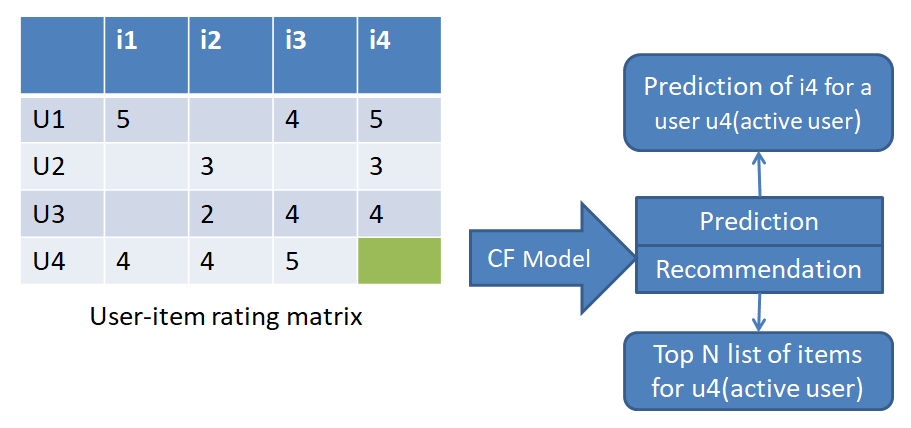
\includegraphics[width=0.9\linewidth]{cf_process1}
	\caption{Collaborative Filtering Process \cite{33}}
	\label{fig:collaborative_process}
\end{figure}


\noindent Collaborative Filtering technique is broadly divided into 2 categories \cite{11}. 
\begin{itemize}
\item Memory-based CF \\
A memory-based collaborative filtering approach predicts item ratings based on ratings given by different users for an item.
\item Model-based CF \\
In contrary to memory-based collaborative filtering, the model-based algorithm takes the data that has been already preprocessed where it is cleansed, filtered, and transformed and generates a learned model to make predictions. This algorithm calculates the similarity between users or items by generating a model and analyzing their pattern to predict ratings on unseen items \cite{28,29,30}.
\end{itemize}

\subsubsection{User-User CF}

In user-user collaborative filtering similarity between users is calculated based on how similarly they rate several items. For any active user, it finds users other than active users whose ratings are similar to the active user and use their ratings on items other than items rated by the active user to predict what active user may prefer. Thus, it recommends items to the users that are most preferred by similar users.
\\
Consider an example of users and ratings given by users for different recipes. This algorithm will find a similarity between each user based on the ratings they have given to the recipes in the past. The prediction of a recipe for a user u is calculated by computing weighted sum of the user ratings given by other users to the recipe i.
The prediction for recipe i is given in \autoref{eq:user-user-cf}

\begin{equation}
P_{u,i} = \frac { \sum_v(R_{v,i} * S_{u,v})}{\sum_v S_{u,v}}
\label{eq:user-user-cf}
\end{equation}
\\
Where, 
\\
\noindent
$P_{u,i} = $ \text{prediction of recipe } $i$ 
\\
$R_{v,i} = $ \text{rating given by user} $v$ \text{ to recipe } $i$ 
\\
$S_{u,v} = $\text{similarity between users.} 
\\

\noindent To predict the ratings for a user other than active user we need to calculate similarity score. The similarity between users can be calculated with the help of several methods described in section \nameref{similarity_methods}. Prior to that, it is important to find items rated by both users and their ratings. Based on those ratings, if we choose to calculate similarities by using Pearson correlation, then we will get a correlation score between users. A higher correlation implies a higher similarity. Recommendations are made based on these predicted values.
\\
This algorithm is quite expensive in terms of time as it involves calculating a similarity score between each user and from that score calculating predictions.
\\

\subsubsection{Item-Item CF}

Item-Item CF filtering can be introduced to solve challenges in User-User CF. As seen in user-user CF may become so expensive if we have a large number of users. If we have a huge number of users than items then it is ideal to adopt item-based CF.
\\
\\
This algorithm calculates the similarity between items instead of users. It considers ratings of the active user to make predictions for item $i$, as $i$ will be similar to the items rated in the past by the active user. Therefore, a user may prefer to use his own ratings than using some other users' ratings. It helps in maintaining user preferences and choices. The similarity between items can be calculated using any method discussed in section \nameref{similarity_methods}.
\\
The rating prediction for item-item collaborative filtering is calculated in \autoref{eq:item-item-cf}
\begin{equation}
P_{u,i} = \frac { \sum_N(S_{i,N} * R_{u,N})}{\sum_N (\vert S_{i,N} \vert)}
\label{eq:item-item-cf}
\end{equation}
\\
Where,
\\
\noindent
$P_{u,i} = $ \text{prediction of item $i$ for user } $u$
\\
$R_{u,N} = $ \text{rating given by user } $u$ \text{ on item } $N$
\\
$S_{i,N} = $\text{similarity between item $i$ and $N$.}
\\
\\

\subsubsection{Singular Value Decomposition (SVD)}
\label{sec:svd}
SVD is a technique of matrix factorization which is used to reduce the number of features in the data set. The matrix factorization is done on the matrix which is generated by the user's feedback in the form of ratings on different items. In SVD, the technique is used to detect a latent relationship between users and items. Then it will generate a low dimensional representation of original matrix space to calculate neighborhood in the reduced space \cite{32}. The original ratings matrix decomposes by SVD in two matrices in such a way that the product of decomposed matrices is the original rating matrix. The SVD is calculated as shown in \autoref{svd}
\begin{equation}
SVD(M) = U \cdot S \cdot V^{T}
\label{svd}
\end{equation}
\noindent Where,\\
$SVD(M)$ denotes matrix M with dimensions $m \times n$ which are total number of users and items respectively.\\
Dimensions of matrix $U$ will be $m \times m$ \\
Dimensions of matrix $S$ will be $m \times r$ \\
Dimensions of matrix $V$ will be $r \times n$ \\
$U$ and $V$ are called left and right singular vectors. To reduce features of dataset one can keep only k highest values of V and S and eliminate lower entries. So, $(r-k)$ columns from $U$ and $(r-k)$ rows from $V^{T}$ are discarded to generate $U_{k}$ and $V_{k}^{T}$ matrices. Now $M_{k}$ can be constructed with multiplication of $U_{k}$ and $V_{k}$ together using $S_{k}$. Generated $M_{k}$ will closest rank $k$ matrix to $M$. Mathematically it can be represented as in \autoref{svd1}

\begin{equation}
M_{k} = U_{k} \cdot S_{k} \cdot V_{k}^{T}
\label{svd1}
\end{equation}

\noindent Rating prediction for user $u$ for item $i$ is given in \autoref{svd2}

\begin{equation}
r_{ui} = r_{u} + U_{k} \sqrt{S_{k}^{T} (u)} \cdot \sqrt{S_k} \cdot V_{k}^{T}
\label{svd2}
\end{equation}

\noindent With SVD we can predict ratings with good accuracy.

\subsubsection{Advantages and Disadvantages of collaborative filtering techniques}
\label{cf_pros_cons}
Collaborative Filtering technique has major advantages over content-based technique in such domains where there is a selection of many features is not necessary. Collaborative filtering has the ability to recommend a new item such that even if the content of that item is not stored as a user's preference in the user's profile. It is a very successful algorithm but it suffers from some drawbacks \cite{10}.
\begin{itemize}
\item Data Sparsity Problem \\
Data sparsity problem is a result of a lack of availability of information about ratings of items in the dataset. A dataset with a huge number of items but only a few of them rated by users leads to a sparse user-item matrix. This problem causes the generation of weak recommendations as locating successful neighbors is difficult.
\item Cold Start Problem \\
Cold-start is a situation where the system does not have enough information about a new user or a new item in order to make relevant predictions. The user profile or item profile will be empty as a user has not rated any item so, the preference of a user will be unknown to the system. In Collaborative filtering, the similarity between users is considered based on a user's ratings.
\item Scalability \\
The nearest neighbor algorithm requires high computations. It grows with a number of users and number of items in the system. Any web-based system which has a huge number of items and users may suffer from high scalability.

\end{itemize}

\subsection{Hybrid Filtering}
Content-based filtering technique do not involve the opinions of all users while recommending items. It has limitations to recommend only those items that are in the range of user's taste as discussed in the \nameref{sec:cb}. However, collaborative filtering cannot give prediction to items that have never been rated as discussed in the \nameref{sec:cf}. Hybrid filtering techniques uses a combination of different recommendation techniques to overcome limitations of pure recommendation techniques and to improve performance \cite{37,38}. The performance of recommendation techniques can be measured by different evaluation metrics as discussed in section \nameref{sec:eval_metrics}. Many researchers have combined content-based and collaborative filtering techniques to gain better results. The idea behind combining different recommendation techniques is that the resultant algorithm will provide more accurate and effective recommendations than any single algorithm \cite{39}. Burk \cite{40} has categorized hybrid techniques in different types. One of them is weighted hybridization.\\

\subsubsection{Weighted Hybridization}
In this technique, the results of multiple algorithms are combined to generate predictions by integrating the scores of each algorithm used. For example, the P-Tango system combines content-based and collaborative filtering techniques \cite{41}. At the start, both techniques were equally weighted but based on performance and user ratings the weight for different techniques has gradually adjusted. In this thesis, the weighted hybrid technique has been used. Similar to the P-Tango system, this thesis combines content-based and collaborative filtering using SVD techniques to overcome the limitations of traditional algorithms. This thesis performed experiments on different weighting factors starting with equal weights but looking at offline evaluation results, weight for content-based and collaborative techniques has gradually adjusted as discussed in section \nameref{sec:hybrid_impl}.



